\documentclass[a4paper]{article}
\usepackage[fontsize=13pt]{scrextend}
\usepackage[utf8]{vietnam}
\usepackage{amsmath}
\usepackage{amsfonts}
\usepackage{xcolor}
\usepackage{titlesec}
\usepackage{mdframed}
\usepackage{amssymb}
\usepackage{pgf,tikz,pgfplots}
\usepackage{graphicx}
\graphicspath{ {../figures/} }
\usepackage{array}
\usepackage{cases}
\usepackage{listings}
\usepackage{tabulary}
\usepackage{color}
\usepackage{float} 
\usepackage{hyperref}
\usepackage{multirow}
\usepackage{minitoc}
\pgfplotsset{compat=1.5}
\usepackage{mathrsfs}
\usetikzlibrary{arrows, calc}
\usepackage{fancyhdr}
\pagestyle{fancy}
\pagestyle{empty}
\usepackage[noend]{algpseudocode}
\usepackage{algorithm,algpseudocode}
\usepackage{lipsum}
\makeatletter
\newenvironment{breakablealgorithm}
  {% \begin{breakablealgorithm}
   \begin{center}
     \refstepcounter{algorithm}% New algorithm
     \hrule height.8pt depth0pt \kern2pt% \@fs@pre for \@fs@ruled
     \renewcommand{\caption}[2][\relax]{% Make a new \caption
       {\raggedright\textbf{\fname@algorithm~\thealgorithm} ##2\par}%
       \ifx\relax##1\relax % #1 is \relax
         \addcontentsline{loa}{algorithm}{\protect\numberline{\thealgorithm}##2}%
       \else % #1 is not \relax
         \addcontentsline{loa}{algorithm}{\protect\numberline{\thealgorithm}##1}%
       \fi
       \kern2pt\hrule\kern2pt
     }
  }{% \end{breakablealgorithm}
     \kern2pt\hrule\relax% \@fs@post for \@fs@ruled
   \end{center}
  }
\makeatother
\definecolor{dkgreen}{rgb}{0,0.6,0}
\definecolor{gray}{rgb}{0.5,0.5,0.5}
\definecolor{mauve}{rgb}{0.58,0,0.82}
\usepackage[
    backend=biber,
    style=numeric,
    natbib=true,
    url=true, 
    doi=true,
    eprint=false,
    sorting=nyt
]{biblatex}
\addbibresource{refs.bib}
\lstset{frame=tb,
  language=Python,
  aboveskip=3mm,
  belowskip=3mm,
  showstringspaces=false,
  columns=flexible,
  basicstyle={\small\ttfamily},
  numbers=none,
  numberstyle=\tiny\color{gray},
  keywordstyle=\color{blue},
  commentstyle=\color{dkgreen},
  stringstyle=\color{mauve},
  breaklines=true,
  breakatwhitespace=true,
  tabsize=3
}
\hypersetup{
    colorlinks=true,
    linkcolor=blue,
    filecolor=magenta,      
    urlcolor=red,
    pdftitle={An Example},
	pdfpagemode=FullScreen,
    }
\renewcommand{\listfigurename}{Danh sách hình}
\renewcommand{\listtablename}{Danh sách bảng}
\newcommand{\tabitem}{~~\llap{\textbullet}~~}
\usepackage[left=2cm,right=2cm,top=2cm,bottom=2cm]{geometry}
\author{Nguyễn Văn Lộc}
\newmdenv[linecolor=black,skipabove=\topsep,skipbelow=\topsep,
leftmargin=-5pt,rightmargin=-5pt,
innerleftmargin=5pt,innerrightmargin=5pt]{mybox}
\begin{document}
\fancyhf{}
\lhead{Báo cáo đồ án môn học Mạng máy tính}
\chead{}
\rhead{Địa điểm yêu thích}
\cfoot{\thepage}
\rfoot{}
\lfoot{}
\pagestyle{fancy}
\renewcommand{\headrulewidth}{0pt}
\renewcommand{\footrulewidth}{0pt}
\begin{titlepage}
\begin{mybox}
\begin{center}
\fontsize{12}{12}\selectfont
\textbf{ĐẠI HỌC QUỐC GIA THÀNH PHỐ HỒ CHÍ MINH}\\
\textbf{TRƯỜNG ĐẠI HỌC KHOA HỌC TỰ NHIÊN}\\
\textbf{KHOA CÔNG NGHỆ THÔNG TIN}
\end{center}
\vskip 1 cm
\begin{figure}[H]
\begin{center}

\includegraphics[scale=0.25]{figures/logo}
\end{center}
\end{figure}
\vskip 1 cm
\begin{center}
\fontsize{18}{14}\selectfont
\textbf{SƯU LIỆU ĐỒ ÁN MÔN HỌC}\\
\fontsize{26}{16}\selectfont
\textbf{MẠNG MÁY TÍNH}\\
\fontsize{18}{12}\selectfont
\textbf{ĐỀ TÀI: Điều khiển máy tính thông qua email}
\end{center}
\vskip 1 cm
\fontsize{14}{12}\selectfont
\textbf{Giảng viên lý thuyết:} Thầy Đỗ Hoàng Cường\\
\textbf{Lớp:} 20TN\\
\textbf{Thành viên thực hiện:}
\begin{itemize}
\item 20120131 $-$ Nguyễn Văn Lộc
\item 20120536 $-$ Võ Trọng Nghĩa
\item 20120572 $-$ Nguyễn Kiều Minh Tâm
\end{itemize}
\vskip 3 cm
\begin{center}
\textbf{THÀNH PHỐ HỒ CHÍ MINH, THÁNG 5-6 NĂM 2022}
\end{center}
\end{mybox}
\end{titlepage}
\tableofcontents
\listoffigures
\listoftables
\newpage
\section{Thông tin của nhóm}
\begin{table}[H]
\begin{center}
\begin{tabular}{|c|c|c|}
\hline 
MSSV & Họ và tên & Công việc \\ 
\hline 
20120131 & Nguyễn Văn Lộc & Bài 1 + 2 \\ 
\hline 
20120536 & Võ Trọng Nghĩa & Bài 4 + \LaTeX \\ 
\hline 
20120572 & Nguyễn Kiều Minh Tâm & Bài 3 + 5 \\ 
\hline 
\end{tabular}
\caption{Bảng phân công thành viên} 
\end{center}
\end{table}

\section{Mức độ hoàn thành}
\textbf{Bài 1:} $100\%$ (5/5)\\
\textbf{Bài 2:} $100\%$ (14/14)
\newpage
\section{Kịch bản giao tiếp của chương trình}
\newpage
\section{Môi trường lập trình và các framework hỗ trợ để thực thi ứng dụng}
\label{env}
\subsection{Hệ điều hành}
Ứng dụng được lập trình trên hệ điều hành Windows 11.
\subsection{Ngôn ngữ và các thư viện}
Ứng dụng được lập trình bằng ngôn ngữ Python 3.\\
Các thư viện sử dụng trong chương trình:
\begin{itemize}
\item Thư viện \texttt{json} dùng để giao tiếp với cơ sở dữ liệu.
\item Thư viện \texttt{socket} cho việc trao đổi dữ liệu giữa client và server.
\item Thư viện \texttt{tkinter}, \texttt{PIL} cho việc xây dựng giao diện.
\item Các thư viện khác: \texttt{queue}, \texttt{logging}, \texttt{random}, \texttt{string}, \texttt{tempfile}, \texttt{hashlib}, \texttt{ctypes}, \texttt{functools}.
\end{itemize}
\newpage
\section{Hướng dẫn sử dụng các tính năng của chương trình}

\subsection{Yêu cầu}
Để sử dụng được chương trình, máy tính phải cài đặt Python 3 và các thư viện ở phần \ref{env}.

\subsection{Khởi động server}
Để khởi động server, ta vào đường dẫn chứa các tập tin mã nguồn của server, mở terminal và sử dụng câu lệnh: \lstinline[language=bash]{python main.py} hoặc \lstinline[language=bash]{python3 main.py}.
\begin{figure}[H]
\center{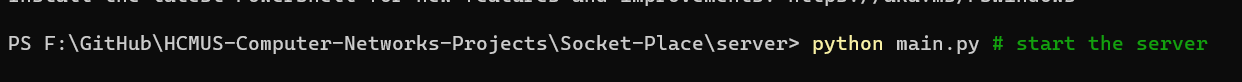
\includegraphics[scale=0.6]{instructions/start_server}}
\caption{Khởi động server}
\end{figure}

\subsection{Khởi động client}
Để khởi động client, ta vào đường dẫn chứa các tập tin mã nguồn của client, mở terminal và sử dụng câu lệnh: \lstinline[language=bash]{python main.py} hoặc \lstinline[language=bash]{python3 main.py}.
\begin{figure}[H]
\center{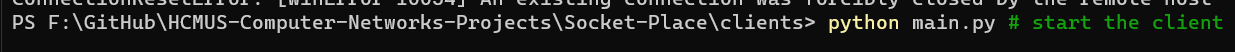
\includegraphics[scale=0.6]{instructions/start_client}}
\caption{Khởi động client}
\end{figure}

\subsection{Giao diện khởi động client}
Sau khi khởi động, client có giao diện như sau:
\begin{figure}[H]
\center{\includegraphics[scale=0.6]{instructions/client_first_gui}}
\caption{Khởi động client}
\end{figure}
Giao diện khởi đầu của client là danh sách các địa điểm đang được server quản lý, các thông tin hiển thị bao gồm: ID địa điểm và tên địa điểm.\\
Trên giao diện khởi đầu, nút \textbf{Xem chi tiết} bên cạnh tên mỗi địa điểm cho phép ta truy vấn thông tin chi tiết về địa điểm đó từ server; nút \textbf{Tải về hình ảnh} bên cạnh mỗi địa điểm cho phép ta tải về các hình ảnh của địa điểm đó từ server, hình ảnh sau khi tải về được lưu trong thư mục \textbf{\textit{Temp}} và được hiển thị lên GUI.\\
Ở phía dưới cùng của giao diện là nút \textbf{Tải tất cả hình ảnh đại diện}, cho phép ta tải về hình ảnh đại diện của tất cả các địa điểm đang được quản lý bởi server. Hình ảnh sau khi tải về được xử lý tương tự bên trên.

\subsection{Truy vấn thông tin chi tiết một địa điểm}
Nút \textbf{Xem chi tiết} ở giao diện khởi đầu cho phép client truy vấn thông tin chi tiết, được lưu tại server, về địa điểm tương ứng. Các thông tin hiển thị lên màn hình gồm: mã số địa điểm, tên địa điểm, tọa độ (vĩ độ, kinh độ) của địa điểm, mô tả và hình đại diện. Hình \ref{query1} là ví dụ về truy vấn thông tin chi tiết một địa điểm.
\begin{figure}[H]
\center{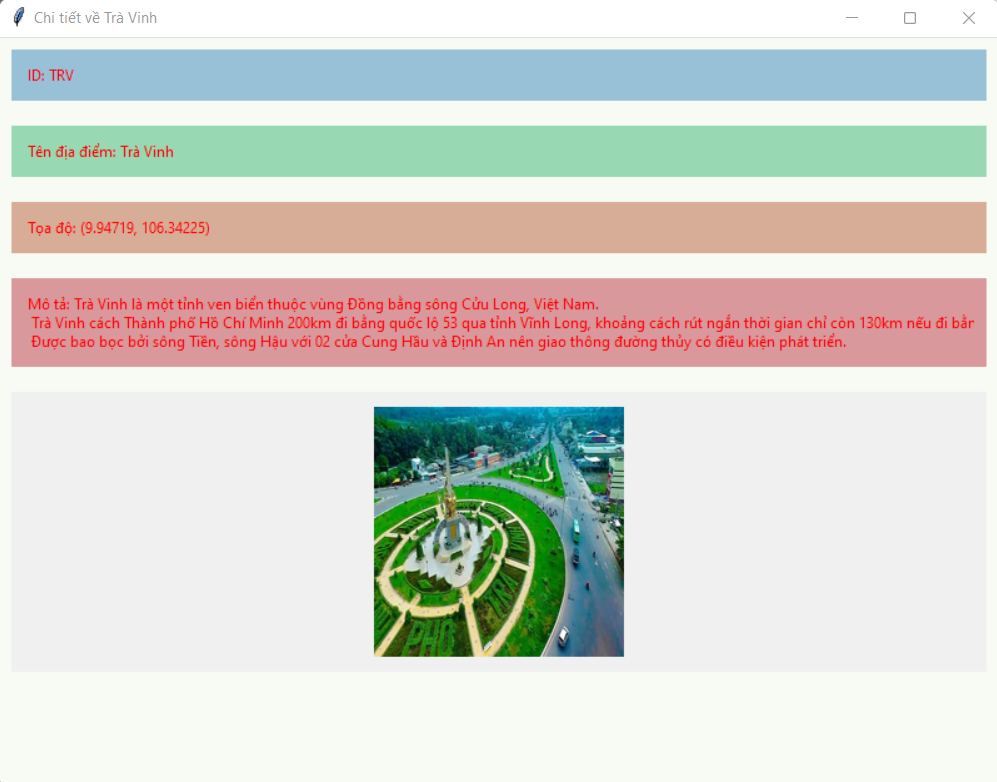
\includegraphics[scale=0.8]{instructions/query_one}}
\caption{Truy vấn thông tin chi tiết một địa điểm}
\label{query1}
\end{figure}

\subsection{Tải tất cả hình ảnh dại diện}
\label{down_all_avt}
Nút \textbf{Tải tất cả hình ảnh đại diện} cho phép client tải về tất cả hình ảnh đại diện của các địa điểm từ server. Hình ảnh sau khi tải về được lưu trong thư mục \textbf{\textit{Temp}} và được hiển thị lên giao diện của client. Các nút \textbf{Hình kế} và \textbf{Hình trước} tương ứng cho ta xem hình ảnh kế tiếp và hình ảnh ngay trước của hình ảnh hiện tại. Hình \ref{all1}, \ref{all2} và \ref{all3} là ví dụ về tải tất cả hình ảnh đại diện.
\begin{figure}[H]
\center{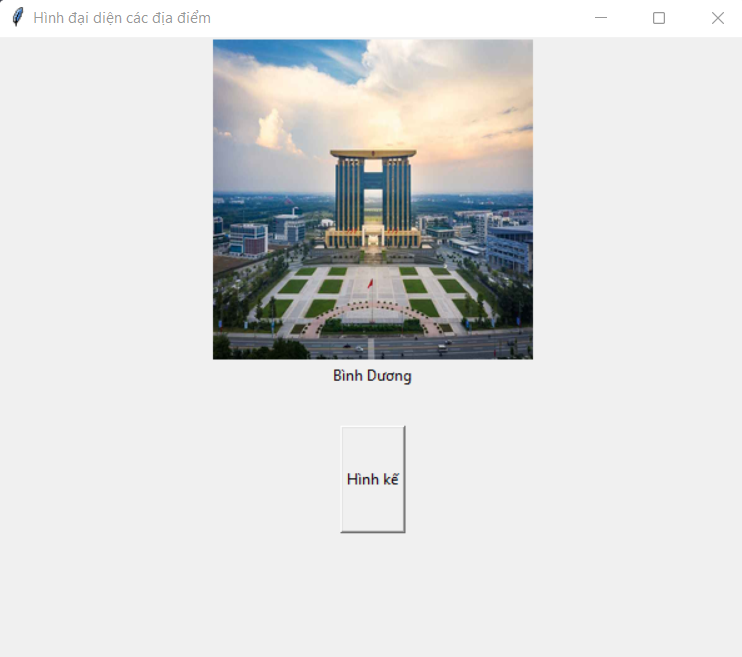
\includegraphics[scale=0.8]{instructions/down_all_avt_1}}
\caption{Tải tất cả hình ảnh đại diện}
\label{all1}
\end{figure}

\begin{figure}[H]
\center{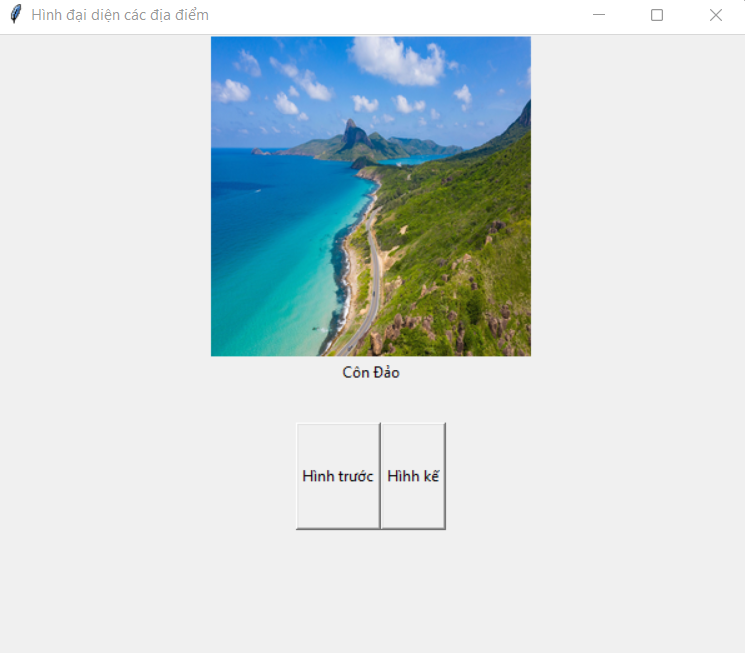
\includegraphics[scale=0.8]{instructions/down_all_avt_2}}
\caption{Tải tất cả hình ảnh đại diện}
\label{all2}
\end{figure}

\begin{figure}[H]
\center{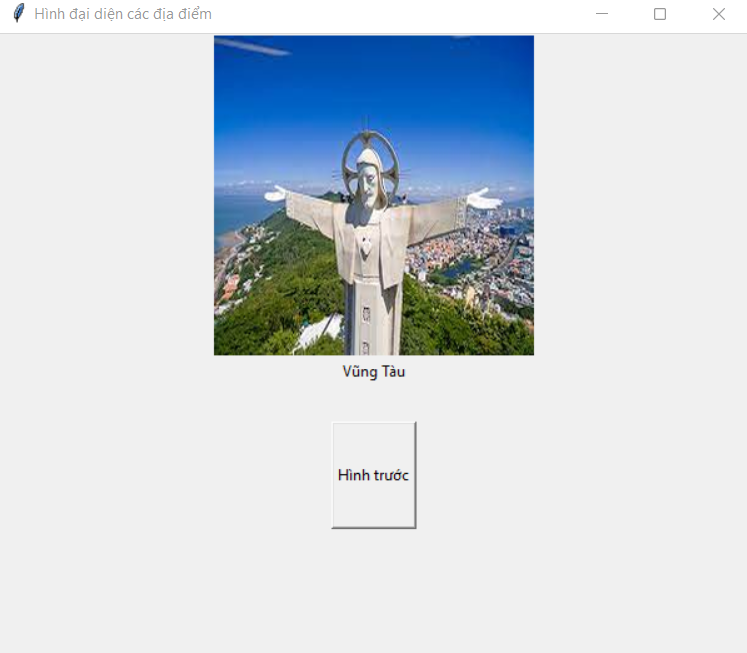
\includegraphics[scale=0.8]{instructions/down_all_avt_3}}
\caption{Tải tất cả hình ảnh đại diện}
\label{all3}
\end{figure}

\subsection{Tải các hình ảnh của một địa điểm}
Nút \textbf{Tải về hình ảnh} bên cạnh mỗi địa điểm cho phép client tải về tất cả hình ảnh của một địa điểm từ server. Hình ảnh sau khi tải về được xử lý tương tự như phần \ref{down_all_avt}. Các nút trong giao diện hiển thị hình ảnh cũng tương tự. Hình \ref{img1}, \ref{img2} và \ref{img3} là ví dụ về tải về các hình ảnh của một địa điểm.
\begin{figure}[H]
\center{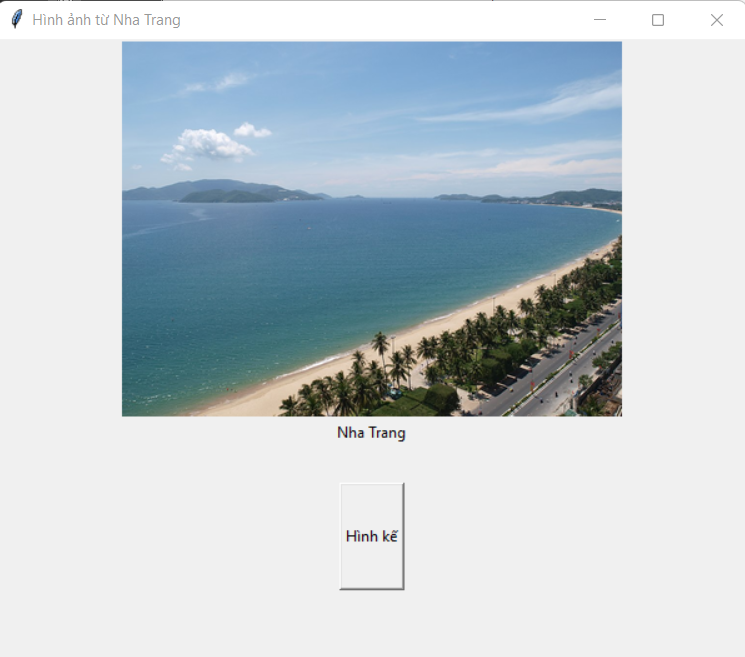
\includegraphics[scale=0.8]{instructions/down_all_img_1}}
\caption{Tải các hình ảnh của một địa điểm}
\label{img1}
\end{figure}

\begin{figure}[H]
\center{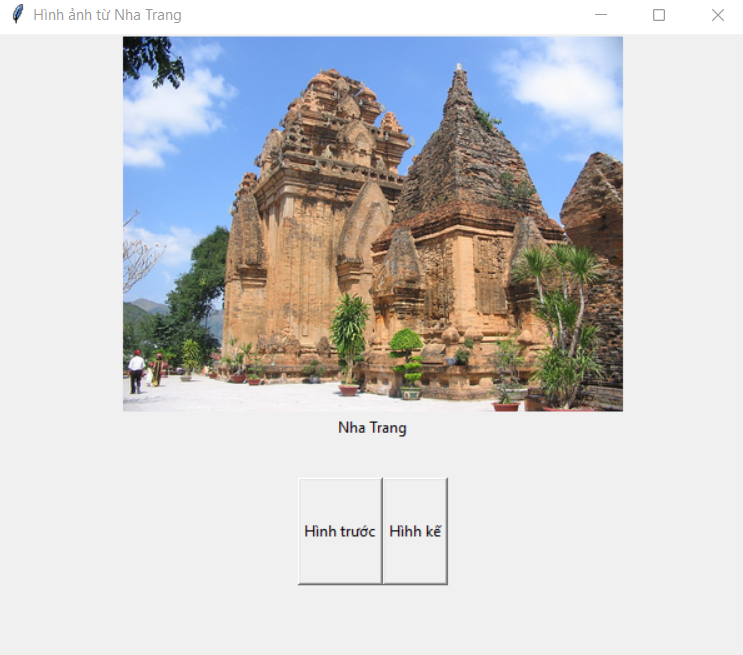
\includegraphics[scale=0.8]{instructions/down_all_img_2}}
\caption{Tải các hình ảnh của một địa điểm}
\label{img2}
\end{figure}

\begin{figure}[H]
\center{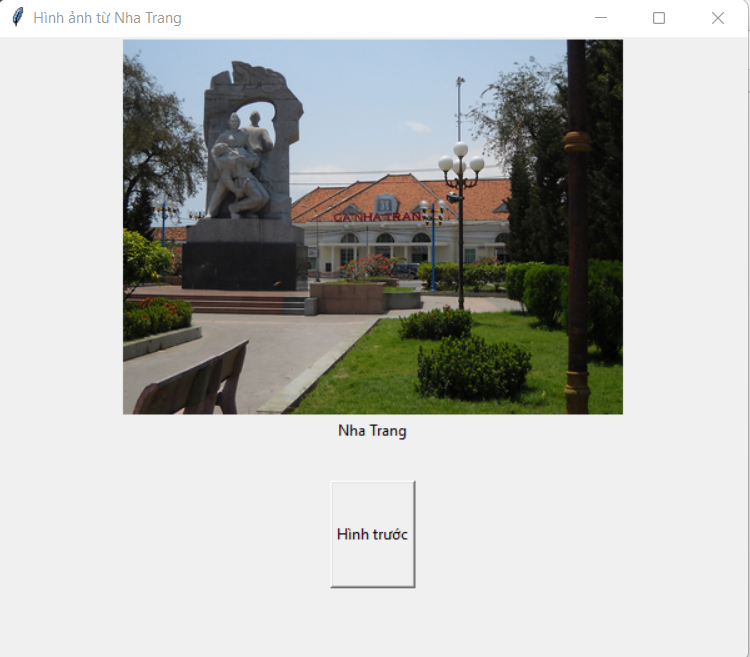
\includegraphics[scale=0.8]{instructions/down_all_img_3}}
\caption{Tải các hình ảnh của một địa điểm}
\label{img3}
\end{figure}

\subsection{Demo}
Demo của chương trình có thể được xem tại \href{https://youtu.be/K0q0q73HTxc}{đây}.\\
Link: \url{https://www.youtube.com/watch?v=K0q0q73HTxc}

\newpage
\section{Phân công công việc}
\begin{table}[H]
\begin{center}
\begin{tabular}{|c|c|p{0.38\textwidth}|c|}
\hline 
MSSV & Họ và tên & Công việc & Phần trăm đóng góp \\ 
\hline 
20120131 & Nguyễn Văn Lộc & Thiết kế các hàm ở client và GUI & 35 \\ 
\hline 
20120536 & Võ Trọng Nghĩa & Thiết kế giao thức truyền dữ liệu giữa client và server & 45 \\ 
\hline 
20120572 & Nguyễn Kiều Minh Tâm & Thiết kế GUI & 20 \\ 
\hline 
\end{tabular}
\caption{Bảng phân công thành viên} 
\end{center}
\end{table}
\nocite{*}
\newpage
\printbibliography[title = Tài liệu tham khảo chủ yếu]
\end{document}